En esta sección desarrollaremos y mostraremos los resultados de los experimentos para:

\begin{itemize}
\item Los protocolos distinguidos.
\item La incidencia de paquetes ARP en la red.
\item Los nodos distinguidos.
\end{itemize}

\section{Experimento incidencia de ARP}

Para poder observar la incidencia de paqueres ARP en la red voy a utilizar una serie de muestras tomadas de distintas redes y graficarlas en un histograma, despues de mostrar
los resultados daremos una explicación del por que de los mismo.

\begin{figure}[ht!]
\centering
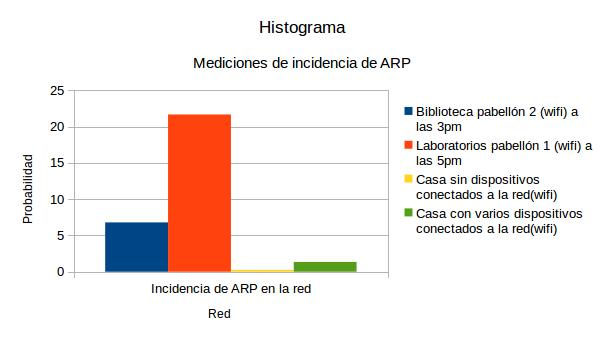
\includegraphics[width=90mm]{imagenes/IncidenciaARP.jpg}
\caption{Comparación de porcentaje de apariciones de ARP en distintas redes o con distintas condiciones.\label{overflow}}
\end{figure}

Como podemos ver la red de los laboratorios tiene más porcentaje de paquetes ARP que el de la biblioteca. Esto se debe a que en el laboratorio del pabellón 1 ingresan 
constantemente personas y, por lo tanto, la mayoría de ellos ingresan en la red a través de las computadoras del mismo o de usando el wifi de estos con sus celulares. Esto 
ocurre en menor medida en la biblioteca ya que no se usan computadoras que no sean propias de los que ingresan, por lo tanto, por la red hay mucho más trafico de paquetes 
ARP en los laboratorios. Además al estar en una red privada, es más común que se efectúen envíos de mensajes entre computadoras y los routers de las mismas.

\begin{comment}
Intento de experimentos1:

Para poder observar la incidencia de paqueres ARP en la red voy a utilizar el buscador de Google Chrome y la función de scapy arping. Usando la interfaz de wlan0 podre sniffear
los paquetes que habra con el buscador y usando arping podre enviar paquetes ARP.\\

Ejecuto  sudo ./capture.py wlan0 entropia-tipos 1000 y, al mismo tiempo, abro el buscador. 

Resultados:

Simbolo 2048 tiene probabilidad 0.996158770807(IP).

Simbolo 34525 tiene probabilidad 0.00128040973111(IPv6).

Simbolo 2054 tiene probabilidad 0.00256081946223(ARP).

La entropia de la fuente es 0.0492085855963.

Simbolo 2048 tiene probabilidad 0.996158770807(IP).

Simbolo 34525 tiene probabilidad 0.00256081946223(IPv6).

Simbolo 2054 tiene probabilidad 0.00128040973111(ARP).

La entropia de la fuente es 0.0398813035719.

Simbolo 2048 tiene probabilidad 0.99875(IP).

Simbolo 2054 tiene probabilidad 0.00125(ARP).

La entropia de la fuente es 0.0138570614629.

Simbolo 2048 tiene probabilidad 0.998740554156(IP).

Simbolo 2054 tiene probabilidad 0.00125944584383(ARP).

La entropia de la fuente es 0.013948087353.

Simbolo 2048 tiene probabilidad 0.985987261146(IP).

Simbolo 34525 tiene probabilidad 0.0101910828025(IPv6).

Simbolo 2054 tiene probabilidad 0.00382165605096(ARP).

La entropia de la fuente es 0.118197558737.

Ejecuto  sudo ./capture.py wlan0 entropia-tipos 100 y, al mismo tiempo, ejecuto arping("192.168.2.0/24").

Resultados:
Simbolo 2048 tiene probabilidad 0.0481481481481(IP).

Simbolo 2054 tiene probabilidad 0.951851851852(ARP).

La entropia de la fuente es 0.278477724908.

Simbolo 2048 tiene probabilidad 0.0769230769231(IP).

Simbolo 34525 tiene probabilidad 0.0244755244755(IPv6).

Simbolo 2054 tiene probabilidad 0.898601398601(ARP).

La entropia de la fuente es 0.554261234655.

Simbolo 2048 tiene probabilidad 0.0115384615385(IP).

Simbolo 2054 tiene probabilidad 0.988461538462(ARP).

La entropia de la fuente es 0.0908278259323.

Simbolo 2048 tiene probabilidad 0.011320754717(IP).

Simbolo 34525 tiene probabilidad 0.00754716981132(IPv6).

Simbolo 2054 tiene probabilidad 0.981132075472(ARP).

La entropia de la fuente es 0.153356025339.

Simbolo 2054 tiene probabilidad 1.0(ARP).

La entropia de la fuente es 0.0.

Ejecuto  sudo ./capture.py wlan0 entropia-tipos 100 y, al mismo tiempo, abro buscador y ejecuto arping("192.168.2.0/24").

Resultados:

Simbolo 2048 tiene probabilidad 0.737424547284(IP).

Simbolo 34525 tiene probabilidad 0.00201207243461(IPv6).

Simbolo 2054 tiene probabilidad 0.260563380282(ARP).

La entropia de la fuente es 0.847640262877.

Simbolo 2048 tiene probabilidad 0.735412474849(IP).

Simbolo 34525 tiene probabilidad 0.00603621730382(IPv6).

Simbolo 2054 tiene probabilidad 0.258551307847(ARP).

La entropia de la fuente es 0.875119992479.

Simbolo 2048 tiene probabilidad 0.761948529412(IP).

Simbolo 34525 tiene probabilidad 0.00183823529412(IPv6).

Simbolo 2054 tiene probabilidad 0.236213235294(ARP).

La entropia de la fuente es 0.807325191625.

Simbolo 2048 tiene probabilidad 0.757518796992(IP).

Simbolo 34525 tiene probabilidad 0.00093984962406(IPv6).

Simbolo 2054 tiene probabilidad 0.241541353383(ARP).

La entropia de la fuente es 0.808024777478.

Simbolo 2048 tiene probabilidad 0.754066985646(IP).

Simbolo 2054 tiene probabilidad 0.245933014354(ARP).

La entropia de la fuente es 0.804768238572.


Ejecuto  sudo ./capture.py wlan0 entropia-tipos 100 y, al mismo tiempo, arping("192.168.2.0/24") y arping("10.4.2.0/27").
\end{comment}